\subsection{Candidate and retained-best decisions in a recent capture}\label{app:recent-admission-trajectory}

The capture in \cref{fig:fw-recent-candidate-retained} retains the latest
500 consecutive complete admission records matched to the per-round audit.
It remains separate from earlier windows: gaps are unjoined and source
binding remains unresolved (\cref{sec:method-status}).

\begin{figure}[tbp]
  \centering
  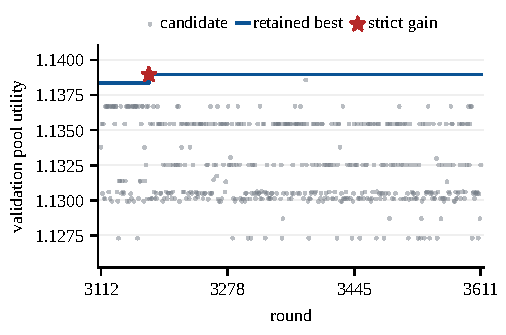
\includegraphics[width=\linewidth]{figures/fig_fw_recent_candidate_retained_trace.pdf}
  \caption{\textbf{One strict gain and 499 rejections occur in rounds \mbox{3112--3611}.}
  Rounds 3112--3611, captured at 10:25 UTC on 2 November 2026.
  Grey points show candidate utility; blue is the post-decision retained
  best (logged dimensionless utility, larger preferred). The star marks
  the one accepted strict gain, at round 3175; the other 499 decisions
  are rejections. Classification uses exact logged values, with no rounding margin.
  These are adaptive decisions on repeatedly used development contexts,
  not independent first-proposal results or evidence of writer or ranking-map lift.
  Scope: \cref{sec:method-status}.}
  \label{fig:fw-recent-candidate-retained}
\end{figure}
